\documentclass[a4paper,12pt]{article}
\usepackage[T1]{fontenc}
\usepackage[utf8]{inputenc}
\usepackage{polski}
\usepackage{color}
\usepackage{graphicx}
\usepackage{amsmath}
\usepackage{amssymb}
\usepackage{hyperref}
\usepackage{float}
\usepackage{listings}
\usepackage[backend=biber]{biblatex}

\addbibresource{bibliografia.bib}

\lstset{
  basicstyle=\ttfamily,
  columns=flexible,
  keepspaces=true,
  literate={ą}{{\k{a}}}1
           {ć}{{\'{c}}}1
           {ę}{{\k{e}}}1
           {ł}{{\l{}}}1
           {ń}{{\'{n}}}1
           {ó}{{\'{o}}}1
           {ś}{{\'{s}}}1
           {ź}{{\'{z}}}1
           {ż}{{\.{z}}}1
           {Ą}{{\k{A}}}1
           {Ć}{{\'{C}}}1
           {Ę}{{\k{E}}}1
           {Ł}{{\L{}}}1
           {Ń}{{\'{N}}}1
           {Ó}{{\'{O}}}1
           {Ś}{{\'{S}}}1
           {Ź}{{\'{Z}}}1
           {Ż}{{\.{Z}}}1
}

\title{Zadanie - wykład 2}
\author{Mikołaj Kubś, 272662}
\date{\today}

\begin{document}

\maketitle

\begin{figure}[H]
  \centering
  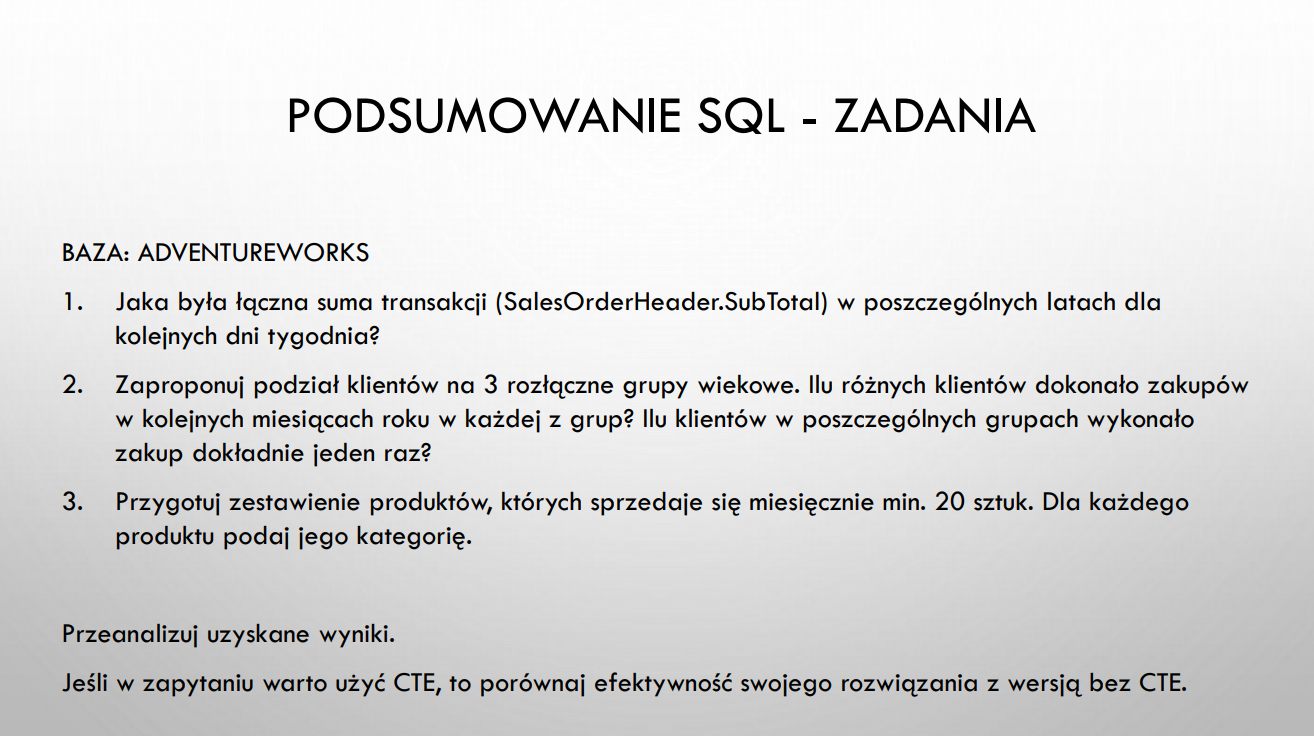
\includegraphics[width=1\textwidth]{images/task1.png}
  \caption{Opis zadań 1-3}
\end{figure}

\begin{figure}[H]
  \centering
  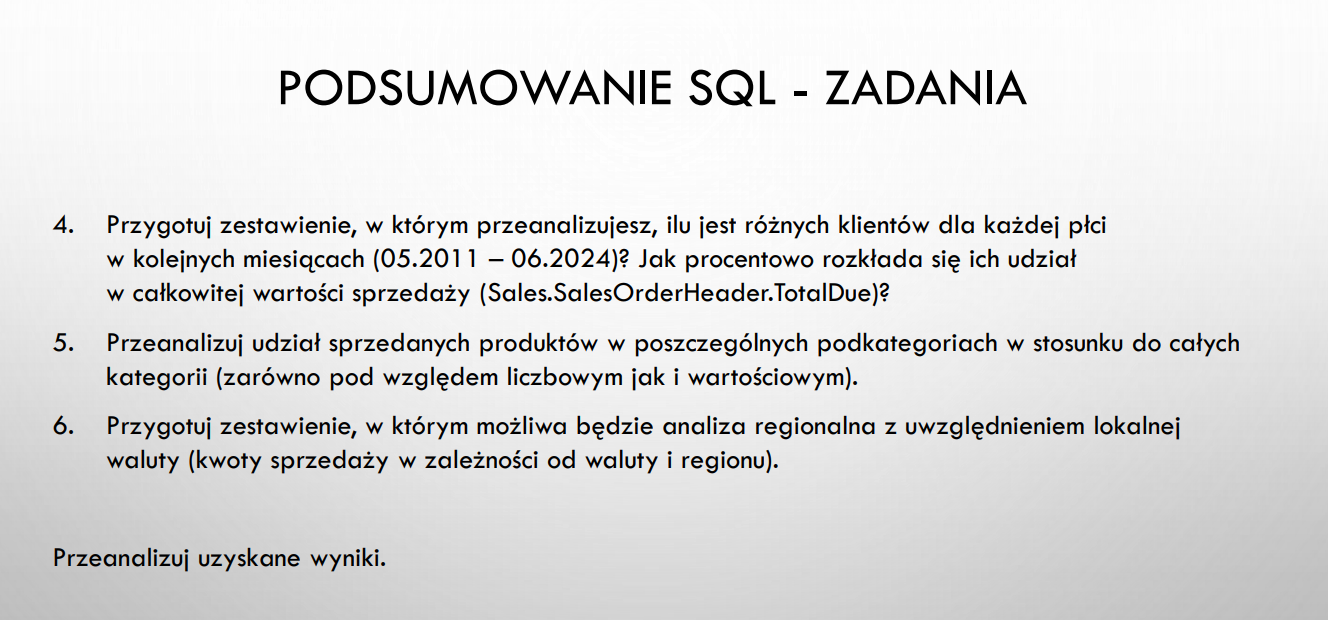
\includegraphics[width=1\textwidth]{images/task2.png}
  \caption{Opis zadań 4-6}
\end{figure}

\section{Kod kwerend}



\end{document}